\section{Conciderations}
\todo{temporary title}
These subsections are had to categorize and insert at the correct place. Perhaps after "Components"

\subsection{Transfer speed}
Faster transfer speed uses more energy, but in a shorter amount of time. Slower transfer speed uses less energy, but over longer time for the nRF24L01. The slower data transfer rate has a significantly longer reach for the nRF24L01, and will therefore be implemented. 

\subsection{Pairing}
In order to add a new node to the network, the node is first needed to be paired up with the main node.
This way, a node could have assigned a unique identity to be able to recognize its sensor readings from other sensors. 
The protocol is described more indepth in \ref{cha:floodingSec}

\subsection{Overloaded nodes}
Nodes close to the main node are prone to receive larger amount of data since many, if not every data packet must go though the node. Looking at \ref{fig:overloadtree} it is seen that node 2 will handle every data packet on its way to the main node. Such low level nodes might be overloaded with data packets, coursing a bottleneck if not thoughtfully spread out. The danger is several higher level nodes are trying to send data packets back to node 2, and node 2 can only handle packets with a certain speed.
\begin{figure}[!h]
	\centering
	\makebox[\textwidth][c]{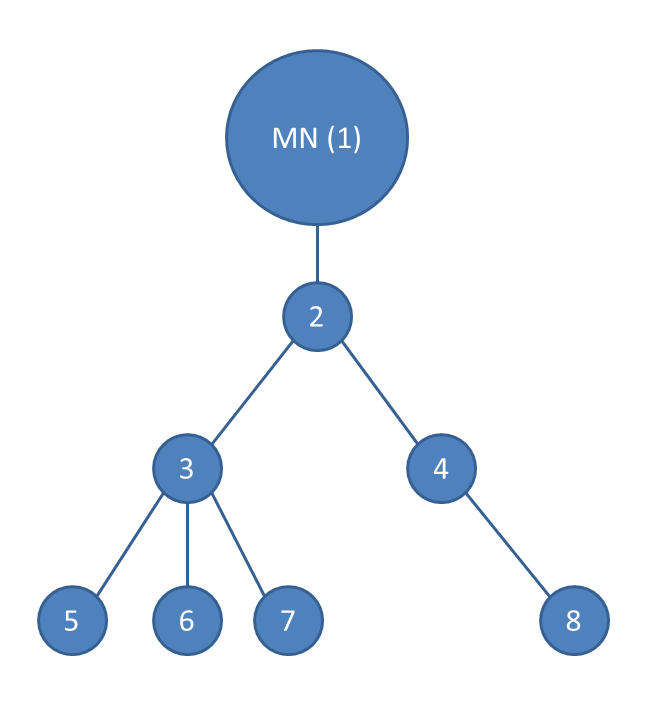
\includegraphics[width=1\textwidth]{chapters/design/figures/overloadtree.png}}
	\caption{Example of a tree.}
	\label{fig:overloadtree}
\end{figure}

\subsection{Data importance}
The gathered data is not critical. If a packet is lost, it is negligible. If the user of the system discovers multiple missing data from a certain area or node, the node can be fixed or replaced.